%%%%%%%%%%%%%%%%%%%%%%%%%%%%%%%%%%%%%%%%%%%%%%%%%%%%%%%%%%%%%%%%%%%%%%%%%%%%%%%%%%%%%%%%%%%%%%%%%%%%%%%
%%%%%%%%%%%%%% Template de Artigo Adaptado para Trabalho de Diplomação do ICEI %%%%%%%%%%%%%%%%%%%%%%%%
%% codificação UTF-8 - Abntex - Latex -                     %%
%% Autor:    Fábio Leandro Rodrigues Cordeiro  (fabioleandro@pucminas.br)                            %%
%% Co-autor: Prof. João Paulo Domingos Silva  e Harison da Silva                                     %%
%% Revisores normas NBR (Padrão PUC Minas): Helenice Rego Cunha e Prof. Theldo Cruz                  %%
%% Versão: 1.0     13 de março 2014                                                                  %%
%%%%%%%%%%%%%%%%%%%%%%%%%%%%%%%%%%%%%%%%%%%%%%%%%%%%%%%%%%%%%%%%%%%%%%%%%%%%%%%%%%%%%%%%%%%%%%%%%%%%%%%
\section{\esp Introdução}

Computadores fazem parte de nosso dia a dia de forma onipresente. Utilizamos nossos dispositivos de forma natural e em diversos formatos: celulares, \textit{tablets}, \textit{smartphones}, computadores de mesa, \textit{notebooks}, etc. Esta diversidade de dispositivos é benéfica e nos oferece novos produtos e soluções a medida que as tecnologias existentes evoluem e novas surgem. Porém a cada novo dispositivo criado, a complexidade para que aplicativos específicos sejam desenvolvidos aumenta e muitas vezes, é um empecilho para sua adoção e disseminação.

Durante muito tempo, a maioria dos aplicativos desenvolvidos era destinado a uma mesma plataforma, por exemplo, computadores de mesa ou dispositivos móveis e algumas vezes para Sistemas Operacionais (SO) diferentes. Caso fosse necessário atender uma nova plataforma ou SO, o aplicativo deveria ser reescrito a partir do zero, muitas vezes em uma linguagem diferente e sem reaproveitar o código existente, para que este novo requisito fosse atendido. Tamanha complexidade dificultou que desenvolvedores mais experientes pudessem utilizar linguagens, ferramentas e técnicas já conhecidas e difundidas para produzir aplicativos, que utilizando o mesmo código, fossem aceitos em mais de uma plataforma.

Com a grande disseminação de tecnologias de computação móvel, como os \textit{smartphones}, este problema se tornou cada vez mais crítico. De acordo com Moore, Van Baalen e Shevchenko (2015), a demanda por aplicações móveis nunca foi tão alta e os desenvolvedores vem sofrendo para criar experiências atrativas nas principais plataformas e atingir os maiores mercados da área. Isso nos mostra, que apesar de efervescente, o mercado não está preparado para atender todas as expectativas dos clientes atuais.

Para encarar este problemas, iniciativas como o Intel XDK, Apache Cordova, Adobe Phonegap e Microsoft Xamarin foram criadas visando permitir o desenvolvimento para múltiplas plataformas de uma forma expansível e customizável, com experiências e funcionalidades específicas em cada uma. 

Atualmente, uma abordagem comum e que possui grande adoção é o empacotamento de \textit{WebApps} em \textit{containers} nativos. Esta abordagem possui duas grandes vantagens: a possibilidade de utilizar diversas bibliotecas e ferramentas já disseminadas e testadas no desenvolvimento web e a facilidade para desenvolvimento e validação do produto desenvolvido, tendo em consideração que o produto final nada mais é do que um \textit{website} com acesso aos recursos do dispositivo por meio do \textit{container} em que foi empacotado. Aplicativos desenvolvidos desta forma são normalmente denominados "híbridos".

Este artigo tem por objetivo principal a elaboração e formalização de uma arquitetura que permita o desenvolvimento de aplicativos híbridos multiplataforma de forma eficaz, possibilitando o uso de diversos padrões e ferramentas já existentes e o reaproveitamento do mesmo código entre plataformas. Como objetivo secundário está a apresentação de um um protótipo, que utilizando da arquitetura elaborada, será capaz de ser distribuído para sistemas \textit{Desktop} tradicionais (Linux, Windows, Mac), dispositivos móveis (iOS, Android, Windows Phone) ou como um site na \textit{WEB} sem alterações em suas camadas internas, mudando apenas a forma de apresentação em cada plataforma, quando necessário.

\section{\esp Referencial Teórico}

Nesta seção serão apresentados fundamentos teóricos do trabalho desenvolvido.

\subsection{\esp Reutilização de Software}

Desde que começamos a desenvolver \textit{software}, estamos buscando formas mais eficientes de fazê-lo. Uma das formas mais eficientes de desenvolver \textit{software} é não desenvolver o que já existe, mas reutilizar padrões e soluções já definidos e testados. 

\cite{pressman2011} diz que componentes reutilizáveis foram criados à medida que a disciplina de engenharia evoluiu, sendo essa uma prática natural em projetos do tipo, enquanto que por outro lado, componentes de \textit{software} reutilizáveis em larga escala, apenas começaram a serem alcançados. Hoje, sistemas complexos devem ser desenvolvidos em prazos muito curtos com uma alta qualidade. Tais exigências, segundo \cite{sommer07}, fizeram com que o desenvolvimento baseado em reuso, se tornasse o padrão para novos sistemas a partir do ano 2000. Tal cenário faz com que os programas escritos devam ser modulares e capazes de se adaptar a diferentes contextos.

A ideia da reutilização, segundo \cite{pressman2011} não é nova, pois vem sendo utilizada desde os primórdios da computação, tendo sua estratégia definida por \cite{unixPhilosophy} há mais de 40 anos. Apesar de existente, antigamente essa rotina era realizada de modo menos organizado e não sendo tratada como princípio ativo do desenvolvimento. O contexto atual exige uma padronização e direcionamento, normalmente tentando-se maximizar a reutilização de \textit{softwares} existentes ou planejando o desenvolvimento, com o reuso acontecendo em tês níveis distintos, definidos por \cite{sommer07}.

\begin{enumerate}
	\item \textbf{Reúso do sistema de aplicação:} Onde a totalidade do sistema pode ser reutilizada sem alterações em outros sistemas via configurações específicas para diferentes clientes.
	\item \textbf{Reúso de Componentes:} Ao reutilizar componentes internos ou subsistemas em diferentes sistemas de informação.
	\item \textbf{Reúso de objetos e funções:} Funções ou componentes que implementa uma única função, como uma função matemática ou uma classe de objetos  podem ser reutilziados na forma de bibliotecas. 
\end{enumerate}

A construção com base em componentes, é, segundo \cite{pressman2011}, o caminho o qual a indústria está trilhando. Apesar da afirmação do autor ainda não possuir comprovação ou dados para validação segundo \cite{cbs28}, o desenvolvimento de componentes reutilizáveis vem recebendo cada vez mais adeptos segundo <PETE BACON WHITE PAPER DO GOOGLE>  e é a abordagem utilizada por esse artigo.

\subsection{\esp Arquitetura de Software}

A Arquitetura de \textit{Software} é uma área da Engenharia de \textit{Software} que visa relacionar e estruturar os componentes e como eles interagem entre si através de interfaces, expondo ao final a estrutura do sistema de uma forma abstrata. É definida por (Len Bass et al., 2012), como:

A arquitetura de um \textit{software} de um programa ou sistema computacional é a estrutura ou estruturas de um sistema, que inclui os elementos de \textit{software}, as propriedades externamente visíveis destes elementos, e os relacionamentos entre eles. Arquitetura é responsável pelas interfaces públicas dos elementos. Seus detalhes privados (detalhes que tenham a ver somente com a implementação interna) não fazem parte da arquitetura.

\section{\esp Metodologia}
Nessa seção as fases do projeto e seus respectivos objetivos são apresentados. Visando melhor separar o processo teórico da implementação prática, três etapas foram definidas e realizadas em sequência.

\subsection{{\it Levantamento dos Requisitos / Identificação do Problema}}
O problema de reuso de \textit{software} foi identificado informalmente pelo autor tendo como principal referência a forma como o desenvolvimento de aplicativos móveis acontece atualmente. Essa necessidade por um reuso de soluções mais amplo foi suportado por outros autores que também já haviam identificado a dificuldade em desenvolver aplicativos móveis e sugerido a utilização da abordagem de desenvolvimento híbrido com alvo em múltiplas plataformas móveis. (Max Lynch, 2014; Adam Bradley, 2013; Sapan Diwakar, 2012; Jose Fermoso, 2009). 

Após a identificação do problema e analisado o cenário atual utilizando as observações oferecidas por \cite{Diwakar2012} foi realizada uma pesquisa das ferramentas de desenvolvimento de software multiplataforma atuais, que se encaixavam no perfil do projeto, com o objetivo de identificar e testar em cada plataforma (\textit{web}, \textit{mobile} e \textit{desktop}), as opções para possível utilização futura. 

\subsection{{\it Especificação da Arquitetura}}

Após pesquisar as ferramentas atuais, teve início a etapa de especificação da Arquitetura sugerida para a resolução do problema identificado. Durante essa etapa, foi produzido um documento contendo a arquitetura sugerida utilizando uma notação de camadas simples.

As camadas finais foram definidas utilizando os conceitos do DBC em conjunto alguns itens da filosofia Unix sugeridos por \cite{unixPhilosophy} e foram levantadas após diversos rascunhos serem produzidos e testes com as ferramentas selecionadas na etapa anterior terem sido testadas. Os testes, em sua maioria, focavam na facilidade em que um mesmo código pudesse ser distribuído dentro dos requisitos definidos pelo projeto e foram essenciais para que a arquitetura, apesar de essencialmente ser um conceito teórico e abstrato, fosse capaz de possuir uma implementação prática. 

A medida em que os testes foram executados algumas arquiteturas sugeridas foram refutadas quando se provaram demasiado complexas, incapazes de extensão ou por se apresentarem incapazes de solucionar o problema especificado. De uma forma geral, o processo de especificação foi interativo e utilizou uma metodologia ágil, o que segundo \cite{pressman2011} oferece uma validação mais rápida.

Após os testes iniciais, as arquiteturas que se provaram teoricamente viáveis foram alinhadas com as ferramentas selecionadas na primeira etapa para que a implementação do protótipo fosse iniciada.

\subsection{{\it Implementação do Protótipo}}

O processo de codificação se baseou nos objetivos adquiridos nas etapas anteriores para realizar a implementação de um protótipo utilizando a arquitetura sugerida. Com base nos testes realizados, foi definido que para uma experiência mais unificada as ferramentas utilizadas utilizariam a mesma linguagem base e possuiriam uma interface programática similar a fim de facilitar a integração entre elas. Uma explicação detalhada da implementação pode ser encontrada em uma seção específica deste artigo.

\section{\esp Tecnologias Utilizadas}
Nessa seção serão apresentadas as tecnologias utilizadas.

\subsection{\esp AngularJS}
\textit{AngularJS} é um \textit{framework} \textit{JavaScript} de código aberto que auxilia a criação de \textit{WebApps}, oferecendo alta performance em múltiplas plataformas e é utilizado por milhões de pessoas ao redor do mundo \cite{angularjs}. Seu foco inicial era facilitar o desenvolvimento e teste de aplicação \textit{single-page} oferecendo uma arquitetura \symbolfootnote[1]MVC/\symbolfootnote[2]MVVM para o \textit{front-end}. Apesar de ainda cumprir muito bem esse papel, vem evoluindo e se solidificando como um dos \textit{frameworks} mais utilizados para desenvolvimento de aplicativos, sejam estes \textit{WEB} ou não \cite{angularjs}. É mantido principalmente por uma equipe do Google e conta com o apoio da comunidade \textit{open-source}. Teve sua primeira versão lançada em Outubro de 2010 e sua próxima evolução, denominada \textit{Angular} 2, a que iremos utilizar para a implementação desse artigo, se encontra em Beta.  

Com a evolução das tecnologias disponíveis juntamente com a crescente complexidade, inerente de \textit{WebApps} modernos, o \textit{framework} adotou em sua nova versão uma forma mais opinativa e declarativa de desenvolvimento baseada em componentes reutilizáveis. Linguagens com mais recursos e de alto nível, com tipagem mais restritiva como \textit{TypeScript} e \textit{Dart}, facilitam a identificação de erros antes de transpilar o código para \textit{JavaScript} e são consideradas alguns dos pontos mais marcantes e \textit{disruptivos} do \textit{Angular} 2.

\footnote{MVC - \textit{\textbf{M}odel \textbf{V}iew \textbf{C}ontroller}}
\footnote{MVVM - \textit{\textbf{M}odel \textbf{V}iew \textbf{V}iew \textbf{M}odel}}

\subsection{\esp Apache Cordova}

O \textit{Apache Cordova} foi criado inicialmente por integrantes da empresa \textit{Nitobi Sofware} em um evento chamado \textit{iPhoneDevCamp} que ocorreu na cidade de São Francisco em 2006. Na época o projeto se chamava \textit{PhoneGap} e foi comprado pela \textit{Adobe Systems} em 2011 \cite{Adobe2011}, um ano após a \textit{Apple} ter confirmado que o \textit{framework} havia sido aprovado como uma forma válida de desenvolvimento de aplicativos para sua loja, a \textit{Apple Store}. De acordo com o documento de aquisição \cite{Adobe2011}, após a compra, a \textit{Adobe} liberou o código fonte para a fundação \textit{Apache}, porém manteve o nome \textit{PhoneGap} como proprietário, a \textit{Apache} então renomeou o projeto como \textit{Apache Cordova}.

O \textit{Cordova} possibilita que desenvolvedores construam aplicações para dispositivo móveis ao empacotar os arquivos HTML, CSS e \textit{JavaScript} em um \textit{container} nativo. Este \textit{container} possui acesso a diversos recursos do dispositivo em que está sendo executado como por exemplo bibliotecas do sistema operacional e recursos de hardware e expõe uma API em \textit{JavaScript} que pode ser consumida pela própria aplicação para acessar esses recursos, não necessitando implementações diferenciadas para plataformas específicas por parte do produto final, ficando isso a cargo da própria biblioteca de \textit{plugins} nativos do \textit{Cordova} \cite{Diwakar2012}.

Por utilizar esta abordagem de empacotamento, os aplicativos criados, apesar de serem distribuídos como código nativo, são considerados híbridos, pois toda a renderização da interface de apresentação é realizada em uma \textit{WebView} (um processo similar ao executado por navegadores para a exibição de páginas \textit{WEB}) e não com componentes nativos da plataforma. Na mesma direção, os aplicativos não são considerados \textit{WebApps}, como um site tradicional, pois além do modo de distribuição diferenciado, possuem acesso as APIs do dispositivo, normalmente bloqueadas para aplicações não-nativas. Essa diferenciação é importante pois possui um impacto significante na performance e fluidez de alguns aplicativos desenvolvidos nesse formato híbrido, tendo em vista que ao utilizar ferramentas web para renderizar a interface, lentidões e perdas de performance podem ser percebidas em comparação com aplicativos totalmente nativos \cite{Diwakar2012}.

De acordo com \cite{CordovaLynch2014}, um dos criadores do \textit{Ionic Framework}, um ponto importante e muito contestado ao utilizar a abordagem de aplicações híbridas com o \textit{Apache Cordova} é a disponibilidade de \textit{plugins} para acessar os recursos nativos. Ao longo da evolução da ferramenta, muitos \textit{plugins} foram criados visando oferecer um acesso transparente as funcionalidades em todas as plataformas, isso faz com que o \textit{Apache Cordova}, ainda de acordo com o autor, seja capaz de realizar a interface com praticamente todo tipo de recurso que o desenvolver necessita na aplicação móvel. A tabela abaixo ilustra bem a grande disponibilidade e variedade de \textit{plugins} e o suporte a cada um nas principais plataformas utilizadas com a ferramenta. 

\begin{table}[]
	\centering
	\caption{Exemplo de recursos disponíveis para algumas plataformas no \textit{Apache Cordova}}
	\label{Meu label}
	\begin{tabular}{|l|l|l|l|l|}
		\hline
	 & Android & Blackberry 10 & iOS  & Windows (8.1, 10) \\ \hline
	Acelerômetro & SIM & SIM & SIM  & SIM \\ \hline
	Estado da Bateria & SIM & SIM &  NÃO  & SIM \\ \hline
	Câmera & SIM & SIM & SIM & SIM \\ \hline
	Captura de Mídia & SIM & SIM & SIM  & SIM \\ \hline
	Compasso & SIM & SIM & SIM  & SIM \\ \hline
	Conexão de Rede & SIM & SIM & SIM & SIM \\ \hline
	Acesso aos Contatos & SIM & SIM & SIM  & PARCIAL \\ \hline
	Versão do Dispositivo & SIM & SIM & SIM  & SIM \\ \hline
	Geolocalização & SIM & SIM & SIM & SIM \\ \hline
	Globalização & SIM & SIM & SIM  & SIM \\ \hline
	Browser InApp & SIM & SIM & SIM & PARCIAL \\ \hline
	Notificações & SIM & SIM & SIM & SIM \\ \hline
	Vibração & SIM & SIM & SIM & PARCIAL \\ \hline
	\end{tabular}
\end{table}

Considerando os diversos benefícios oriundos da utilização do \textit{Apache Cordova}, diversas ferramentas foram construídas o utilizando como base, oferecendo uma camada adicional de abstração e produtividade. \textit{Ionic Framweork} e \textit{Telerik Platform} são alguns exemplos de ferramentas já difundidas no mercado. No decorrer desse artigo, o \textit{Apache Cordova} será utilizado indiretamente para facilitar o acesso aos recursos nativos por meio do \textit{Ionic Framework}.
\subsection{\esp Ionic Framework}

\textit{Ionic} é um \textit{framework JavaScript} de código aberto. Criado no final de 2012, é hoje a tecnologia multiplataforma mais popular para aplicativos móveis, tendo sido utilizado na criação de 1.3 milhões de aplicativos apenas em 2015 \cite{ionic2015}. De acordo com \cite{ionicFIT}, um dos criadores da ferramenta, o foco do \textit{ Ionic Framework} é aprimorar a interface do usuário ao oferecer uma série de bibliotecas com elementos HTML, CSS e \textit{JavaScript} pré-compilados e otimizados para dispositivos móveis. A ferramenta utiliza todas as vantagens do \textit{Apache Cordova} e tenta suprir a necessidade dos aplicativos possuírem elementos de interface similares aos que os usuários já estão acostumados em cada plataforma. Ainda nas palavras do autor, o \textit{framework} possui outros objetivos como promover padrões de design recomendados e documentar melhores práticas.

Os projetos criados com o \textit{framework} utilizam, por padrão, o \textit{AngularJS} visando facilitar o desenvolvimento de aplicações mais robustas. Diferentemente do primeiro, que oferece uma extensa gama de funcionalidades para diferentes necessidades, o \textit{Ionic Framework} foca em oferecer componentes de interface e interação com o usuário para que a experiência de uso respeite o alto padrão de qualidade que os usuários esperam de aplicativos nativos atualmente \cite{ionicFIT}. Algumas de suas funções são a renderização otimizada de listas, criação de formulários com componentes nativos, customização e padronização dos elementos para a plataforma em que o aplicativo esteja executando, transição entre páginas e identificação de recursos por meio de API's simplificadas.

Um exemplo de como alguns componentes oferecidos pelo \textit{framework} se adaptam para plataformas diferentes é ilustrado na Figura \ref{fig:figura1}.

\begin{figure}[ht]
	\centering	
	\caption[\hspace{0.1cm}Comparativo de telas em diferentes dispositivos.]{Comparativo de telas em diferentes dispositivos}
	\vspace{-0.4cm}
	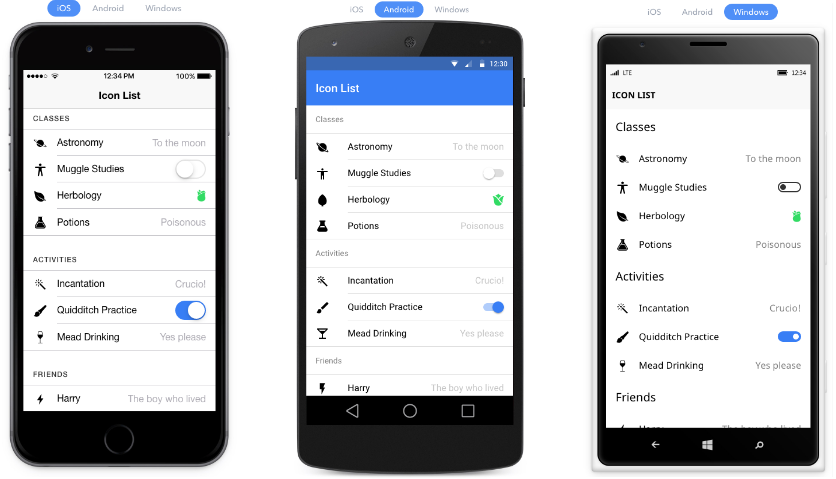
\includegraphics[width=0.6\textwidth]{figuras/ComparativodeTelasIonic.png}
	% Caption centralizada
	% 	\captionsetup{justification=centering}
	% Caption e fonte 
	\vspace{-0.2cm}
	\\\textbf{\footnotesize Fonte: \cite{pressman2011} }
	\label{fig:figura1}
\end{figure}
\vspace{-0.5cm}


\subsection{\esp Electron}

\textit{Electron} é um \textit{framework} \textit{JavaScript} de código aberto que possibilita o empacotamente de \textit{websites} em aplicações nativas ao utilizar o motor de renderização \textit{Chromium} em conjunto com outras tecnologias. Apesar de ser uma tecnologia relativamente nova, vem se concretizando no mercado e recebeu no ano de 2015, 1.2 milhões de downloads \cite{electron}. O \textit{framework} possui opções para gerar aplicativos nativos para os sistemas Mac, Windows e Linux de forma transparente para o usuário final e sem que o desenvolvedor necessite implementar por si só atualizações automáticas, menus nativos, geração de instaladores e outras funcionalidades que, normalmente, são extenuantes em um ciclo de desenvolvimento \textit{desktop} tradicional. \cite{electron}

\subsection{\esp WebSockets}

De acordo com a especificação da \cite{htmlStandard} a interface de \textit{WebSockets} foi introduzida para permitir que aplicações \textit{WEB} mantenham comunicações bidirecionais e persistentes com processos sendo executados em servidores remotos.

Na arquitetura cliente-servidor tradicional, no qual a \textit{WEB} foi construída, as conexões utilizam um padrão HTTP multiplexado, onde é de responsabilidade do cliente iniciar a conexão e requisitar dados, enquanto que a responsabilidade do servidor é atender essas requisições e retornar os dados solicitados. Esse paradigma foi, durante muitos anos, a única forma no qual as aplicações web conseguiam transmitir dados entre a aplicação cliente e o servidor. Com a especificação da interface de \textit{WebSockets}, é possível que conexões persistentes sejam criadas conectando o cliente e servidor, possibilitando que ambas as partes iniciem a transmissão de dados a qualquer momento.

De acordo com a RFC 6455 \cite{ieeeSE} a comunicação de \textit{WebSockets} se inicia com um \textit{handshake} e da mesma forma que o paradigma anterior, o cliente envia uma requisição HTTP com a única adição de um cabeçalho adicional do tipo \textit{Upgrade}. Este cabeçalho informa ao servidor que o cliente deseja estabelecer uma conexão do tipo \textit{WebSocket} e caso a requisição seja aceita e o servidor ofereça suporte a esse tipo de protocolo, a conexão bidirecional é estabelecida e ambos os lados podem iniciar a transmissão de dados , que são transmitidos por meio de mensagens baseadas em \textit{frames}.

%Atualmente, o suporte a WebSockets por navegadores é de 87.65% (Can I Use, ) porém muitas vezes servidores de proxy ou firewall administrativos podem bloquear a transmissão de mensagens por meio do protocolo. Visando uma maior abrangência e tolerância a falhas, esse artigo irá utilizar a bibllioteca SocketIO, que além de WebSockets, implementa outros protocolos de transmissão como JSONP, Flash Messages, Polling, Long-polling, entre outros ( Socket.IO, ).

\section{\esp Implementação}

Nessa seção será detalhada a arquitetura e as ferramentas utilizadas na abordagem.

\subsection{{\it Arquitetura}}

A arquitetura foi divida em três camadas principais, a fim de desacoplar e separar melhor o conceito e responsabilidade de cada uma. São elas:

\begin{enumerate}
	\item \textbf{Componentes:} Definição e Implementação dos componentes
	\item \textbf{Aplicação:} Integração dos componentes 
	\item \textbf{\textit{Deploy}:} Empacotamento do projeto para distribuição
\end{enumerate}

Essas camadas funcionam de forma unidirecional, sempre passando o resultado da anterior para a próxima, sendo que os componentes definidos e implementados são eventualmente integrados e por fim empacotados para distribuição em plataformas específicas. Com essa abordagem o projeto pôde ser desenvolvido de forma modular, pois cada camada não precisa se preocupar com a responsabilidade das demais e por serem implementadas de forma separada cada uma pode ser substituída por uma implementação diferente sem que o fluxo sofra consequências negativas.

\subsubsection{{\it Camada de Componentes}}

Nessa camada, os componente são definidos e implementados utilizando \textit{TypeScript}, um \textit{superset} da linguagem \textit{JavaScript} que oferece suporte a classes, interfaces, tipagem explícita, entre outras funcionalidades não suportadas pela versão atual do \textit{JavaScript} (ES5).

Ao utilizar essas funcionalidades os componentes implementados podem ser compartilhados de forma mais simples e provêm maior facilidade na sua reutilização por terem em sua definição um formato mais explícito.

Os componentes desenvolvidos foram separados em dois grupos principais, seguindo a abordagem sugerida por\cite{presentContainerAbramov} em componentes de apresentação e composição. Os componentes de apresentação são responsáveis por como os dados são apresentados e possibilitam um maior nível de reutilização por não salvarem nenhum estado próprio. Já os componentes de composição se preocupam em definir e implementar como as ações são tratadas e os dados se comportam internalmente . Geralmente implementações desse tipo são compostas por sub-componentes de apresentação. 

Durante a implementação dessa camada, foi possível perceber os benefícios das tecnologias escolhidas. O \textit{TypeScript} permitiu o uso de \textit{decorators} juntamente com classes utilizando injeção de dependência para criação dos componentes, o que fez com que a codificação ficasse mais explícita e simples, possibilitando um maior nível de abstração e a utilização de metadados para configuração. A abordagem de tipagem explícita também se provou útil ao possibilitar inspeções do código sem a necessidade de execução do interpretador de \textit{JavaScript} e que se alinhou de forma eficaz com a utilização de módulos, uma funcionalidade que durante a implementação do projeto ainda não possui suporte amplo pela versão atual do \textit{JavaScript}. A separação do código em módulos permitiu que a reutilização se tornasse mais clara pois cada componente pôde ser separado em seu próprio módulo. Essa prática só foi adotada após algumas refatorações e se provou útil quando a aplicação começou a crescer pois cada componente utiliza o princípio de responsabilidade única e possui sua própria lógica, independente dos demais.

A utilização de conceitos de programação funcional também foram essenciais para a codificação eficiente desta camada. A minimização de efeitos colaterais com ampla utilização de funções puras, que utilizam o conceito de imutabilidade de parâmetros e possuem comportamento previsíveis, permitiu que os componentes implementados possuíssem comportamentos e escopos mapeados, fazendo com que sua reutilização se tornasse mais eficaz ao encapsular seu funcionamento interno e não modificando o escopo em que foram inseridos.

\subsubsection{{\it Camada de Aplicação}}

Essa camada é responsável por integrar os componentes implementados na anterior de tal maneira que o produto final possua uma árvore de componentes interconectados que possam representar a aplicação final. Essa proposta é a recomendação oficial da biblioteca utilizada, \textit{AngularJS} e também respeita o paradigma de desenvolvimento baseado em componentes \cite{pressman2011}.

Além da integração dos componentes de forma estrutural, essa camada também é responsável pelo tratamento de mensagens externas e o encaminhamento de forma normalizada desses dados para outras partes da aplicação por meio do controle de estados.

Nessa camada foi também definido a arquitetura de estado da aplicação. Por utilizar \textit{WebSockets} para comunicação externa, a aplicação necessita ser capaz de tratar diversos eventos assíncronos, além da simples entrada de dados por meio de formulários. Isso fez com que uma estrutura de estados utilizando o padrão de projeto\textit{ Publish/Subscribe} fosse implementada a fim de propagar e publicar tais eventos por toda a aplicação, porém, após os testes iniciais, foi detectado que muitas vezes os estados de variáveis independentes em partes distintas da aplicação não estavam sendo mantidos em sincronia. Esse fator, em adição à necessidade constante do desenvolvedor final sempre ser responsável por adicionar tratadores de eventos a fim de tratar tais mudanças, fez com que esse padrão de projeto fosse substituído por uma implementação que utiliza os conceitos de uma abordagem denominada \textit{Redux}.

Esta abordagem utiliza alguns conceitos do padrão \textit{Publish/Subscribe} e adiciona algumas definições imperativas a fim de prover, seguindo a própria documentação, um gerenciamento de estados com comportamento previsível e que possibilite traçar uma linha do tempo das mudanças realizadas ao utilizar conceitos como imutabilidade e funções puras \cite{redux}.

A abordagem também utiliza o conceito de ações explícitas e todas as mudanças de estados devem possuir uma ação correspondente que, por sua vez, deve ser emitida a fim de notificar as partes interessadas do evento ocorrido. Esta comunicação utiliza uma abordage top-down de forma que todas as ações enviadas criam um novo estado que é repassado para todos os componentes, para que estes possam reagir da forma como foram definidos \cite{redux}.

De uma forma geral, essa camada é uma abordagem abstrata que foca na composição dos componentes para que os mesmos, quando implementados na camada anterior, possam ser altamente reutilizáveis, necessitando apenas serem importados no local desejado para que possam ser utilizados. Isso permite que uma extensa gama de componentes possa existir e que o desenvolvimento da aplicação em si seja apenas a combinação destes de uma forma funcional, o que, como já foi dito, é um dos princípios do DBC.

\subsubsection{{\it Camada de Deploy}}
A camada final é a responsável por empacotar a solução implementada e incluir as funcionalidades necessárias para que essa possa ser executada em todas as plataformas suportadas. Isso é realizado utilizando \textit{scripts} pré-determinados para cada plataforma com o intuito de possibilitar customizações específicas para cada uma delas, caso necessário. 

Apesar ser responsável apenas pelo empacotamento, essa camada possui diferentes implementações por si só, tendo em vista que algumas plataformas não aceitam a combinação de HTML + CSS + \textit{JavaScript} para interpretação de forma nativa ou limitam recursos quando executados via \textit{WebView}. Esta limitação exigiu que arquivos próprios fossem criados visando a execução da aplicação nessas plataformas. Isso foi identificado ao decorrer da implementação quando ao gerar o projeto final da aplicação para empacotamento, era necessário adicionar \textit{scripts} extras para que a plataforma conseguisse identificar a página como um \textit{WebApp}. No caso do \textit{Ionic Framework}, as plataformas suportadas na versão 2 não apresentaram esse problema, porém algumas vezes aplicações executando versões mais antigas na plataforma \textit{Android} 4.4 ou inferior necessitaram ser embarcadas com um navegador próprio, a fim de viabilizar a identificação de diversos recursos nativos, aprimorar a performance e possibilitar um funcionamento transparente para o usuário final.

De forma similar, quando a aplicação foi inicialmente preparada para distribuição em computadores de mesa utilizando a ferramenta \textit{Electron}, foi identificado a necessidade de adicionar arquivos e configurações extras a fim de permitir a renderização correta. O que foi identificado é que a ferramenta utiliza, fundamentalmente, duas \textit{threads}, sendo uma responsável pelo código da aplicação e outra pela renderização do HTML. Essa separação, apesar de útil e performática, necessita um arquivo extra e configurações específicas para identificar momentos em que a aplicação necessita ser renderizada novamente, como por exemplo ao receber eventos assíncronos via \textit{WebSockets} quando fora de foco. Tal peculiaridade fez com que um \textit{script} mais elaborado fosse desenvolvido a fim de permitir que as aplicações distribuídas por esse meio funcionassem da mesma forma que em aplicações sem essa separação de \textit{threads}.

Durante a evolução do projeto essa camada foi a que mais sofreu alterações pois diversas vezes foi necessário alterar os \textit{scripts} a fim de padronizar o processo de empacotamento de cada plataforma, chegando até a quase se tornar um ponto que poderia refutar a arquitetura por falta de ferramentas que permitissem sua implementação prática. Isso fez com que uma pesquisa mais aprofundada em ferramentas de automação fosse realizada e após uma refatoração com base nas lições aprendidas e com a adoção da ferramenta \textit{Gulp} que trabalha com \textit{Streams} de dados, foi possível implementar \textit{scripts} expansíveis que possibilitaram o reuso de soluções e a padronização de tratamentos para casos específicos, fazendo com que a camada funcionasse de forma eficiente.

\subsection{{\it Principais funcionalidades}}

A ferramenta construída durante a implementação desse artigo, oferece como funcionalidade principal o compartilhamento e exibição em tempo real de \textit{links} entre os dispositivos conectados.
Os \textit{links} compartilhados irão apresentar uma breve descrição e uma imagem de exibição escolhida por inferência ao fazer uma breve análise dos metadados da página. Cada \textit{link} também irá possuir um indicador do tipo de plataforma de origem e qual usuário foi responsável por seu compartilhamento.

\subsection{{\it Estrutura de Comunicação}}

A comunicação entre os dispositivos conectados se dará por meio de eventos emitidos através de uma comunicação bidirecional com o \textit{back-end} por meio de \textit{WebSockets}. A figura a seguir exemplifica as interfaces utilizadas para identificar as mensagens transmitidas, sendo que todas as mensagens ,quando recebidas, serão tratadas e despachadas para os componentes responsáveis utilizando nossa arquitetura \textit{Redux}. 

As interfaces representadas na figura \ref{fig:figura2} tem como objetivo principal facilitar e formalizar o formato no qual os dados serão enviados nas mensagens transmitidas via \textit{WebSockets}.

\begin{figure}[ht]
	\centering	
	\caption[\hspace{0.1cm}Diagrama com as interfaces das mensagens transmitidas via \textit{WebSockets} na aplicação.]{Diagrama com as interfaces das mensagens transmitidas via \textit{WebSockets} na aplicação}
	\vspace{-0.4cm}
	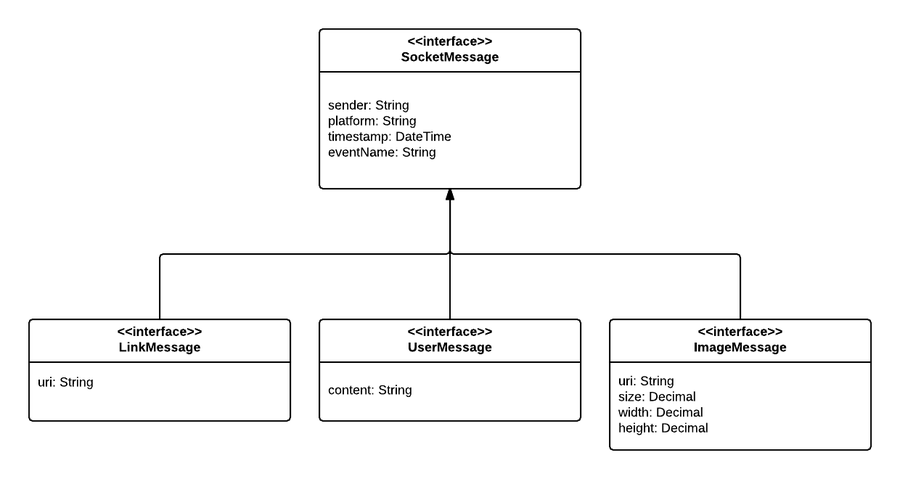
\includegraphics[width=0.6\textwidth]{figuras/SocketInterfaces.png}
	% Caption centralizada
	% 	\captionsetup{justification=centering}
	% Caption e fonte 
	\vspace{-0.2cm}
	\\\textbf{\footnotesize Fonte: \cite{pressman2011} }
	\label{fig:figura2}
\end{figure}
\vspace{-0.5cm}

\subsection{{\it Principais Componentes}}
Seguindo a explicação da camada de componentes, essa seção tem por objetivo explicar de forma mais detalhada como se deu a codificação e identificação dos componentes desenvolvidos para o protótipo.

Com a utilização do\textit{ Ionic Framework}, foram desenvolvidos alguns componentes que representam as páginas da aplicação. Esses componentes podem ser identificados no código por meio do \textit{decorator \textbf{@Page}} e tem por objetivo definir a composição de uma página da aplicação. Esses componentes foram separados em pastas distintas que contêm, no mínimo, um arquivo \textbf{.html} para definição da estrutura da página utilizando \textit{tags} HTML e componentes próprios com a linguagem de \textit{template} do \textit{AngularJS}, um arquivo \textbf{.scss} que é utilizado pelo pré-processados de CSS, \textit{Sass}, para a definição da folha de estilo da página e um arquivo \textbf{.ts} onde a classe que implementa a página é definida utilizando o \textit{TypeScript}. Essa separação por pastas permite trabalhar com estes componentes de páginas de forma modular e faz com que todo o código e folhas de estilo sejam tratados como privados, ou seja, não afetam as outras partes da aplicação, o que normalmente não acontece em aplicações web tradicionais.

Alguns exemplos de componentes de página desenvolvidos no código são: \textit{HomePage, LoginPage e CreatorModalPage}.

\begin{figure}[ht]
	\centering	
	\caption[\hspace{0.1cm}Exemplo de código da página de Login.]{Exemplo de código da página de Login}
	\vspace{-0.4cm}
	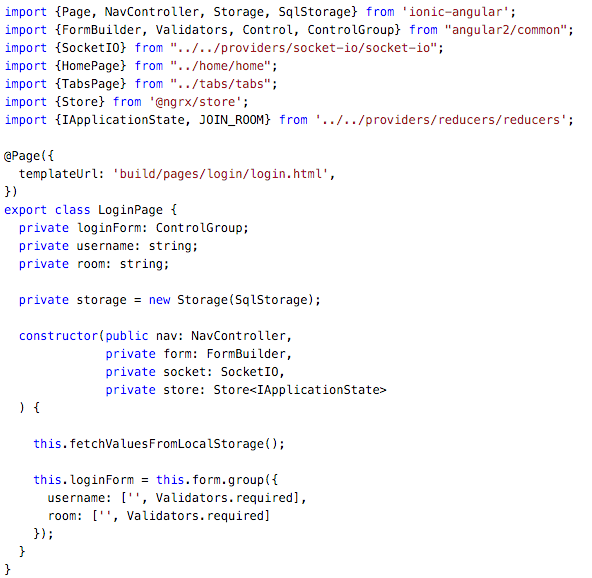
\includegraphics[width=0.6\textwidth]{figuras/CodigoLogin.png}
	% Caption centralizada
	% 	\captionsetup{justification=centering}
	% Caption e fonte 
	\vspace{-0.2cm}
	\\\textbf{\footnotesize Fonte: \cite{pressman2011} }
	\label{fig:figura3}
\end{figure}
\vspace{-0.5cm}

Seguindo esse mesmo modelo modular, diversos outros componentes foram criados em pastas distintas ainda respeitando os conceitos sugeridos por \cite{presentContainerAbramov} de forma a otimizar a reutilização. Durante a implementação do projeto, foi possível identificar que os componentes menores eram reutilizados em maior quantidade e que a composição de componentes se provou mais útil do que a extensão dos mesmos. Esse fato apoia os conceitos da abordagem do DBC e fez com que a abstração, encapsulamento e modularização estivessem no cerne dos componentes desenvolvidos.

Alguns exemplos de componentes desenvolvidos são: \textit{UrlPreview, UrlContentPreview, UrlImagePreview, UrlMessageForm, UrlList, WelcomeMessageCard, NewMessageButton.}

\subsection{{\it Telas do Protótipo}}
Adicionar prints

\begin{figure}[ht]
	\centering	
	\caption[\hspace{0.1cm}Exemplo de código da página de Login.]{Exemplo de código da página de Login}
	\vspace{-0.4cm}
	
\includegraphics[width=0.6\textwidth]{figuras/ExemploTela.png}
	% Caption centralizada
	% 	\captionsetup{justification=centering}
	% Caption e fonte 
	\vspace{-0.2cm}
	\\\textbf{\footnotesize Fonte: \cite{pressman2011} }
	\label{fig:figura3}
\end{figure}
\vspace{-0.5cm}

print

\section{\esp Conclusão}

Com o desenvolvimento bem sucedido do protótipo utilizando a arquitetura sugerida, é possível concluir que o desenvolvimento de aplicações híbridas multiplataformas utilizando o mesmo código compartilhado é viável e possui capacidade para ser utilizada em diversas aplicações.

Com a utilização das ferramentas existentes nas etapas aqui registradas foi possível desenvolver uma solução expansível que possuíse uma certa gama de funcionalidades úteis e não totalmente simplórias de uma forma satisfatória. O nível de customização e qualidade final de renderização e reutilização também foram aceitáveis, indicando que a arquitetura utilizada possa servir de base para outras aplicações em variados contextos.

De uma forma geral, a arquitetura, apesar de expansível e modular, só foi testada com uma certa gama de ferramentas específicas em cada camada, ficando a substituição de cada ferramenta um trabalho futuro a fim de aprimorar o desacoplamento e diminuir as dependências da arquitetura em ferramentas específicas, focando mais em conceitos de responsabilidades do que implementações específicas.
